\documentclass[12pt]{article}

\usepackage{graphicx}
\graphicspath{{../Fichier_Image}}

\title{Hypothèse 3.(b) Porte Bureaux Petits}
\author{Thibault Clodion}

\begin{document}

\maketitle % Permet d'afficher le titre, l'author etc

\underline{Hypothèse :} Les petits bureaux doivent avoir qu'une seule porte pour diminuer le temps de sortie
\newline\newline
\underline{Expérience :}A partir de la 4., faire des simulations avec 1, 2, 3 portes par bureaux. (on concluera en se basant sur les observations aussi)
\newline
Si ils n'ont besoin que d'une porte c'est pour éviter que cela deviennent des couloirs de circulations étroits qui créeraient des ralentissements.
\newline\newline

On consideraque les bureaux petits sont les suivants
\newline\newline
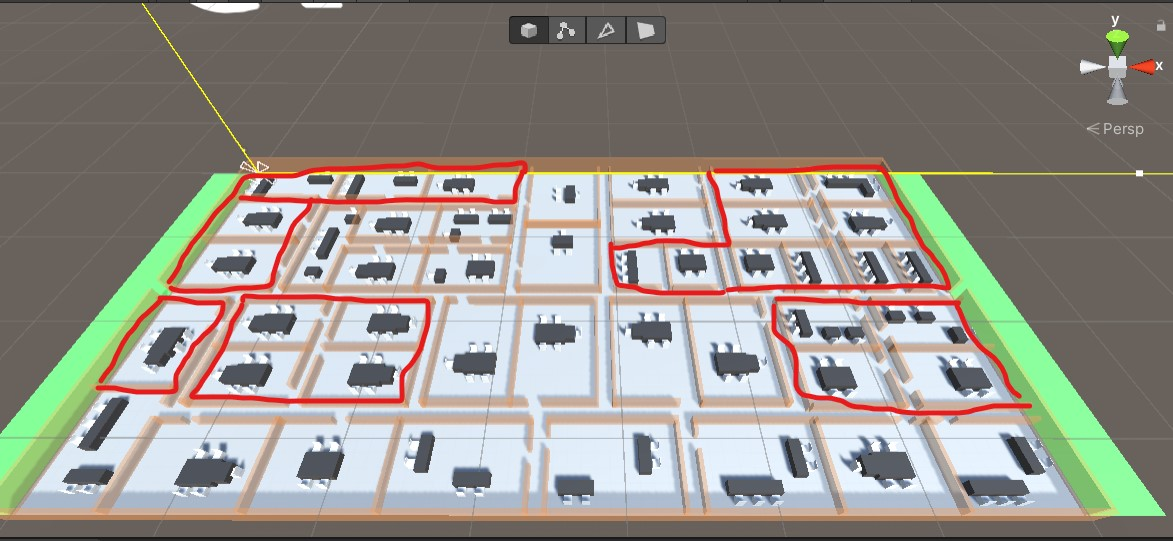
\includegraphics[scale=0.5]{3.(b) Bureaux petits.jpg}
\newline\newline

3.(b) 4. avec 1 porte
\newline\newline
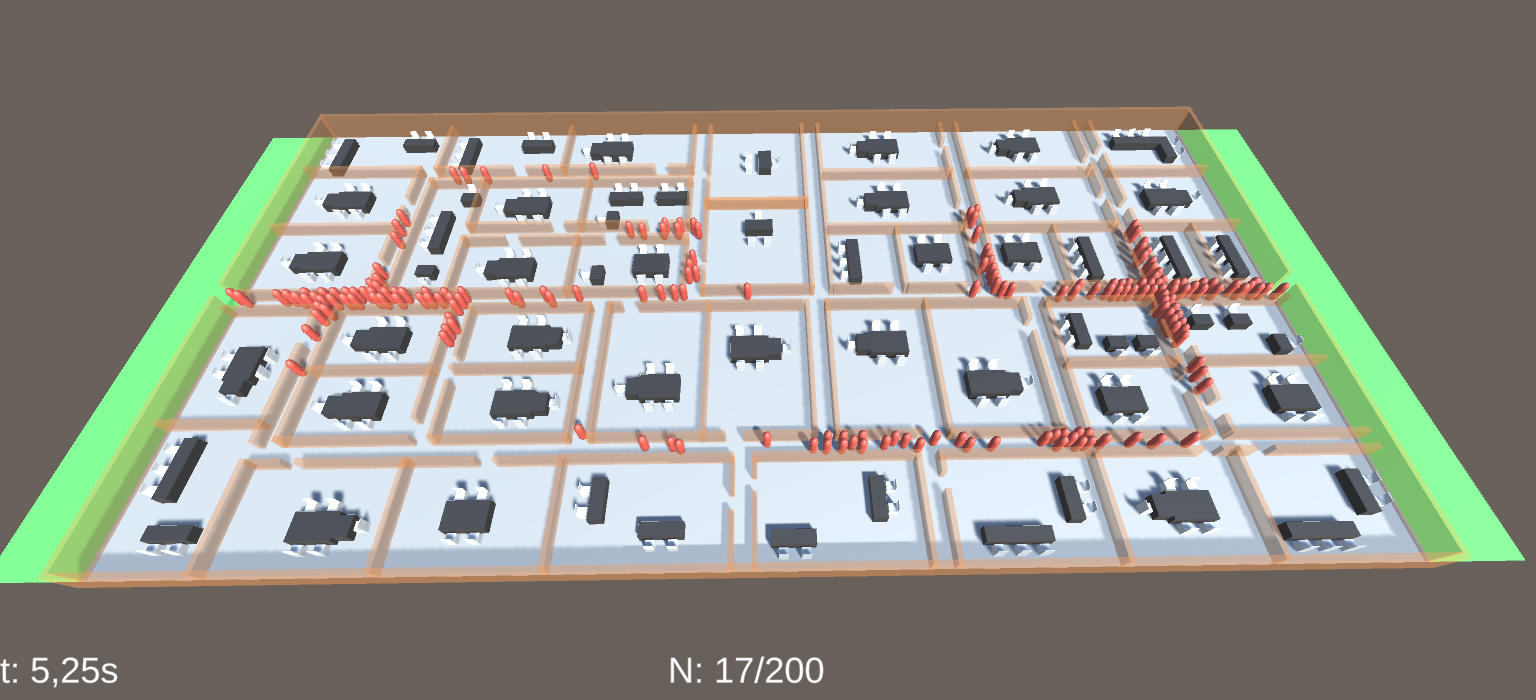
\includegraphics[scale=0.3]{3.(b) 4. avec 1 porte.png}
\newline\newline
Temps moyen de dernière sortie : 23.62s
\newline
$\hspace*{0.2cm}$- Tout le monde sort de son bureau et personne ne rentre dans un autre étant donné qu'ils n'ont qu'une porte. On peut donc réguler le flux et prévoir les chemins de sortie de chacun.
\newline
$\hspace*{0.2cm}$- Tout le monde se retrouve alors bloqué dans les couloirs mais pas dans des petits bureaux (à voir lequel est le mieux)
\newline\newline

3.(b) 4. avec 2 portes
\newline\newline
Temps moyen de dernière sortie : 23.83s
\newline
$\hspace*{0.2cm}$- Création de nouveau chemin et convergence vers les portes plus rapides (mais le phénomène reste limité)
\newline
$\hspace*{0.2cm}$-
\newline\newline

3.(b) 4. avec 3 portes
\newline\newline
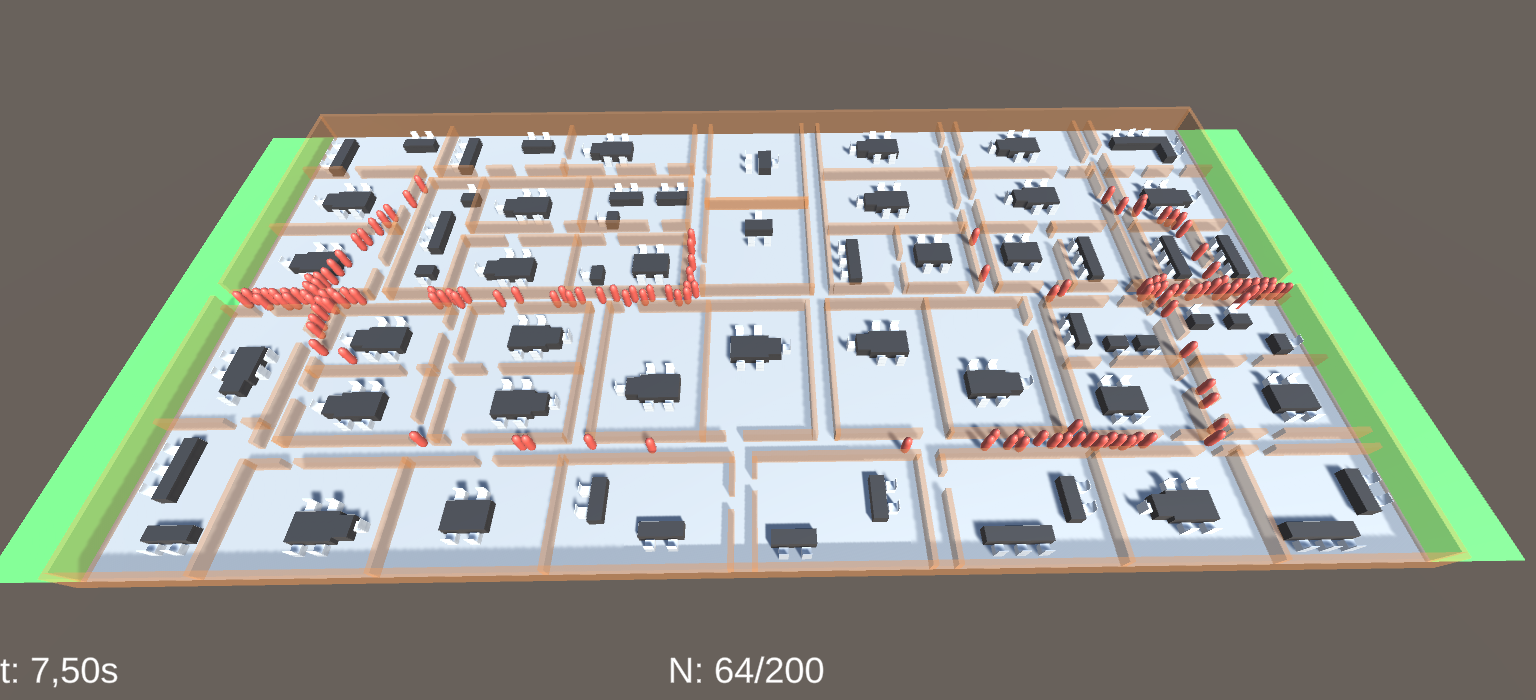
\includegraphics[scale=0.3]{3.(b) 4. avec 3 portes.png}
\newline\newline
\newline\newline
Temps moyen de dernière sortie : 23.73s
\newline
$\hspace*{0.2cm}$- On voit ici la création de plusieurs chemins, les gens circulent dans les bureaux régulièrement.
\newline\newline

\section{Resultat}
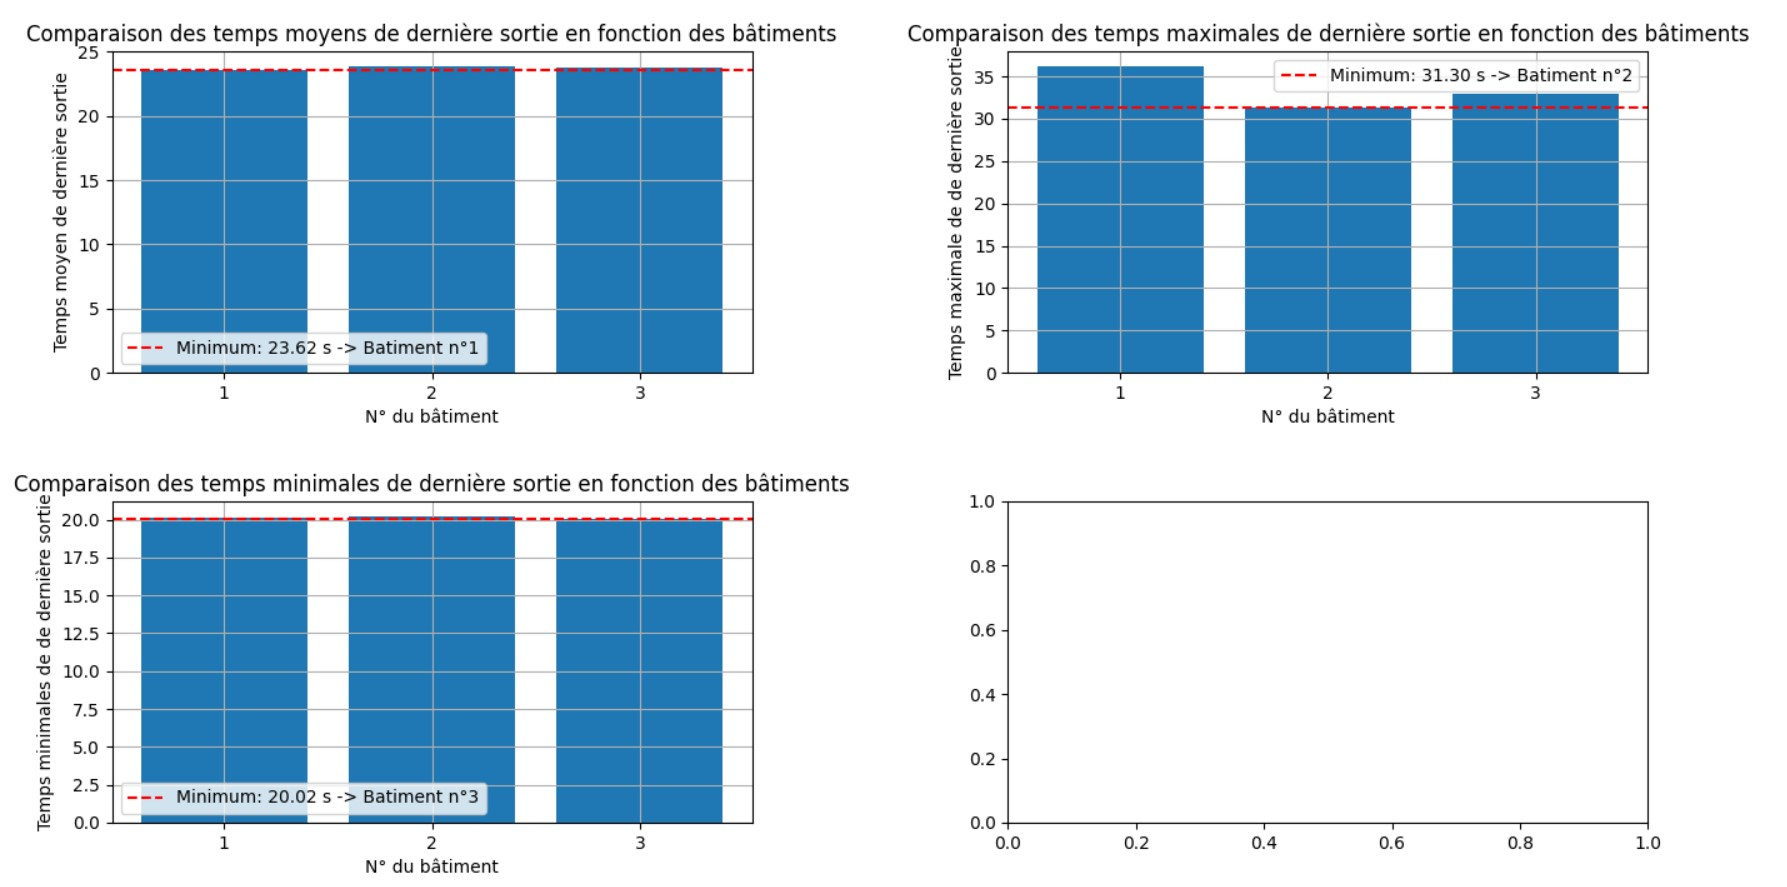
\includegraphics[scale=0.4]{3.(b) Resultat.jpg}
\newline\newline

Effectivement comme attendu, ce sont lorsque les petits bureaux n'ont qu'une porte que le temps est minimale. (Cependant ce n'est pas si net que ça donc il faudra peut-être passer au cas par cas pour certains
bureaux).

\end{document}